\documentclass[a4paper]{report}
\usepackage{times}
\usepackage[pdftex]{graphicx}
\usepackage{hyperref}
\usepackage[cmex10]{amsmath}
\usepackage[font=footnotesize]{subfig}
\usepackage{url}

\begin{document}
\title{Design and Realization of a Digital Predistorter for a Power Amplifier}

\author{Jules Hammenecker \\ Brussels Faculty of Engineering \\ Vrije Universiteit Brussel - Universit\'e Libre de Bruxelles}
\date{2014-2015 }

\maketitle
\begin{abstract}

\end{abstract}

\tableofcontents
\chapter{Introduction}
	\section{Why Digital Predistortion?}
	Power amplifiers are used in almost all wireless communication devices. They amplify the communication signal such that a good signal to noise ratio is obtained. They also are an important power consuming block in a communication chain. A power amplifier is often operated in a nonlinear operation mode to improve its efficiency. This nonlinear behavior should be compensated in a later step to reach the strict telecommunication requirements.
	A Digital Pre-Distortion (DPD) is a common technique to linearize the input-output behavior of a power amplifier. With DPD the input signal of the amplifier is modified such that the desired (i.e. linear) behavior is obtained. 

	\section{Current Techniques of DPD}
	\section{ILC}
	\section{Using ILC for DPD}
		\subsection{}

		A nonlinear dynamic system can alternatively be represented by the combination of a linear transfer function $G_{BLA}$ and a nonlinear function F.
		\begin{figure}[hbtp]
			\centering
			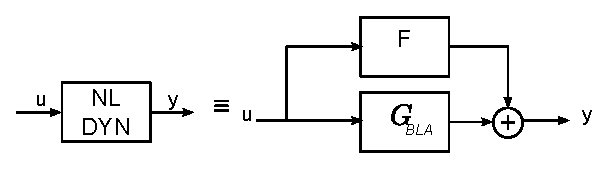
\includegraphics{images/lego1}
			\caption{Alternative representations of a nonlinear system. }
		\end{figure}
	
		\begin{figure}[hbtp]
			\centering
			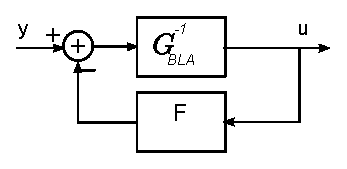
\includegraphics{images/lego2}
			\caption{Switching the input and output, creating the inverse of the nonlinear system. }
		\end{figure}

		\begin{figure}[hbtp]
			\centering
			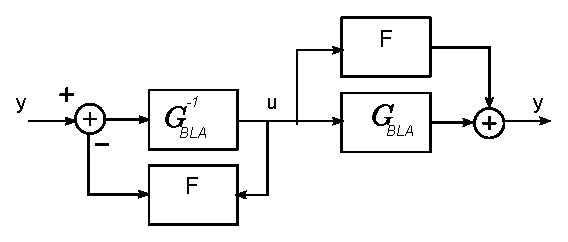
\includegraphics{images/lego3}
			\caption{Connecting the inverse and the original system together. }
		\end{figure}

		\begin{figure}[hbtp]
			\centering
			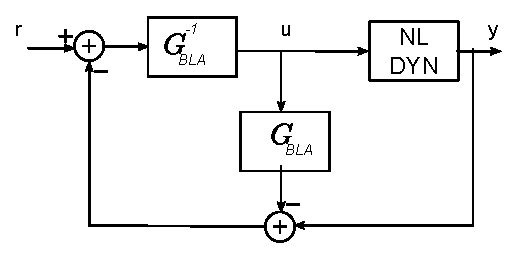
\includegraphics{images/lego4}
			\caption{Getting creative with the blocks. }
		\end{figure}

		\begin{figure}[hbtp]
			\centering
			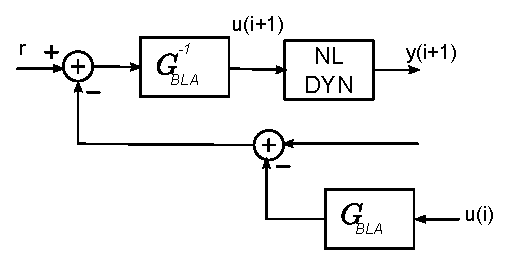
\includegraphics{images/lego5}
			\caption{Cut the loop! }
		\end{figure}

		\begin{figure}[hbtp]
			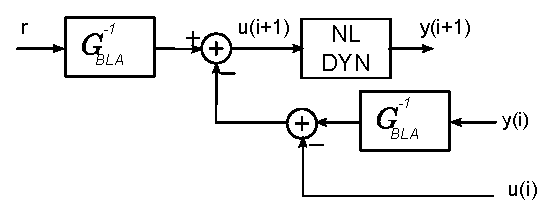
\includegraphics{images/lego6}
			\caption{Reorganise the blocks one last time. }
		\end{figure}


\chapter{Compensating with ILC using the BLA}
\chapter{Estimating the DPD}
\chapter{Results}	

\begin{thebibliography}
	{09}
	
	\bibitem{100ex} J.~Schoukens, R.~Pintelon, Y.~Rolain , \emph{Mastering System Identification in 100 Exercises.}\hskip 1em plus 0.5em minus 0.4em\relax IEEE Press (2012), 183-238. 

\end{thebibliography}

\end{document}
